%   Copyright 2012 Comet Engineering, Patrick Haring & Christian Bürgi
%
%   Licensed under the Apache License, Version 2.0 (the "License");
%   you may not use this file except in compliance with the License.
%   You may obtain a copy of the License at
%
%       http://www.apache.org/licenses/LICENSE-2.0
%
%   Unless required by applicable law or agreed to in writing, software
%   distributed under the License is distributed on an "AS IS" BASIS,
%   WITHOUT WARRANTIES OR CONDITIONS OF ANY KIND, either express or implied.
%   See the License for the specific language governing permissions and
%   limitations under the License.

\documentclass[fontsize=12pt,
               paper=a4,
               twoside=false,
               parskip=half,
               ]{scrartcl}

% Load the packages
%   Copyright 2012 Comet Engineering, Patrick Haring & Christian Bürgi
%
%   Licensed under the Apache License, Version 2.0 (the "License");
%   you may not use this file except in compliance with the License.
%   You may obtain a copy of the License at
%
%       http://www.apache.org/licenses/LICENSE-2.0
%
%   Unless required by applicable law or agreed to in writing, software
%   distributed under the License is distributed on an "AS IS" BASIS,
%   WITHOUT WARRANTIES OR CONDITIONS OF ANY KIND, either express or implied.
%   See the License for the specific language governing permissions and
%   limitations under the License.

% Packages Template
% =================
% 
% Contains packages used for project documentation
% 
% @author burgc5
% 
% To use this simply enter: %   Copyright 2012 Comet Engineering, Patrick Haring & Christian Bürgi
%
%   Licensed under the Apache License, Version 2.0 (the "License");
%   you may not use this file except in compliance with the License.
%   You may obtain a copy of the License at
%
%       http://www.apache.org/licenses/LICENSE-2.0
%
%   Unless required by applicable law or agreed to in writing, software
%   distributed under the License is distributed on an "AS IS" BASIS,
%   WITHOUT WARRANTIES OR CONDITIONS OF ANY KIND, either express or implied.
%   See the License for the specific language governing permissions and
%   limitations under the License.

% Packages Template
% =================
% 
% Contains packages used for project documentation
% 
% @author burgc5
% 
% To use this simply enter: %   Copyright 2012 Comet Engineering, Patrick Haring & Christian Bürgi
%
%   Licensed under the Apache License, Version 2.0 (the "License");
%   you may not use this file except in compliance with the License.
%   You may obtain a copy of the License at
%
%       http://www.apache.org/licenses/LICENSE-2.0
%
%   Unless required by applicable law or agreed to in writing, software
%   distributed under the License is distributed on an "AS IS" BASIS,
%   WITHOUT WARRANTIES OR CONDITIONS OF ANY KIND, either express or implied.
%   See the License for the specific language governing permissions and
%   limitations under the License.

% Packages Template
% =================
% 
% Contains packages used for project documentation
% 
% @author burgc5
% 
% To use this simply enter: \input{./packages.tex}

\usepackage[utf8]{inputenc}
\usepackage[T1]{fontenc}

% Set font to latin modern
\usepackage{lmodern}

\usepackage[pdftex]{graphicx}
\usepackage{epstopdf}

% Create links in pdf documents
\usepackage[colorlinks,pdfpagelabels,pdfstartview=FitH,bookmarksopen=true,bookmarksnumbered=true,linkcolor=black,plainpages=false,hypertexnames=false,citecolor=black] {hyperref}
\hypersetup{
    colorlinks,%
    citecolor=black,%
    filecolor=black,%
    linkcolor=black,%
    urlcolor=black
}
\urlstyle{same}

% Use \enquote{} to create quotation marks
\usepackage{csquotes}

% Create professional tables with booktabs
% @see http://en.wikibooks.org/wiki/LaTeX/Tables#Professional_tables
\usepackage{booktabs}

% Customizable enumerates/itemizes
\usepackage{enumitem}

% git meta information
\usepackage{gitinfo}


\usepackage[utf8]{inputenc}
\usepackage[T1]{fontenc}

% Set font to latin modern
\usepackage{lmodern}

\usepackage[pdftex]{graphicx}
\usepackage{epstopdf}

% Create links in pdf documents
\usepackage[colorlinks,pdfpagelabels,pdfstartview=FitH,bookmarksopen=true,bookmarksnumbered=true,linkcolor=black,plainpages=false,hypertexnames=false,citecolor=black] {hyperref}
\hypersetup{
    colorlinks,%
    citecolor=black,%
    filecolor=black,%
    linkcolor=black,%
    urlcolor=black
}
\urlstyle{same}

% Use \enquote{} to create quotation marks
\usepackage{csquotes}

% Create professional tables with booktabs
% @see http://en.wikibooks.org/wiki/LaTeX/Tables#Professional_tables
\usepackage{booktabs}

% Customizable enumerates/itemizes
\usepackage{enumitem}

% git meta information
\usepackage{gitinfo}


\usepackage[utf8]{inputenc}
\usepackage[T1]{fontenc}

% Set font to latin modern
\usepackage{lmodern}

\usepackage[pdftex]{graphicx}
\usepackage{epstopdf}

% Create links in pdf documents
\usepackage[colorlinks,pdfpagelabels,pdfstartview=FitH,bookmarksopen=true,bookmarksnumbered=true,linkcolor=black,plainpages=false,hypertexnames=false,citecolor=black] {hyperref}
\hypersetup{
    colorlinks,%
    citecolor=black,%
    filecolor=black,%
    linkcolor=black,%
    urlcolor=black
}
\urlstyle{same}

% Use \enquote{} to create quotation marks
\usepackage{csquotes}

% Create professional tables with booktabs
% @see http://en.wikibooks.org/wiki/LaTeX/Tables#Professional_tables
\usepackage{booktabs}

% Customizable enumerates/itemizes
\usepackage{enumitem}

% git meta information
\usepackage{gitinfo}



\begin{document}

% Document title for title.tex
\newcommand{\doctitle}{Design Model}
% Titlepage Template
% ==================
% 
% @author burgc5
% 
% To use this simply enter: % Titlepage Template
% ==================
% 
% @author burgc5
% 
% To use this simply enter: % Titlepage Template
% ==================
% 
% @author burgc5
% 
% To use this simply enter: \input{./title.tex}
% 
% You have to define the commands '\doctitle' and '\docrevision' to give the 
% document a title and a revision on its titlepage.
% Do this with the following command:
% \newcommand{\doctitle}{Document title goes here}
%
% SVN:
% ----
% You also have to define the variables:
% \SVN $Date$
% \SVN $Revision$
%
% As executing the following command on the file:
% > svn propset svn:keywords "Date Revision" filename.tex
% 
% This titlepage needs:
% \usepackage[pdftex]{graphicx}
% \usepackage{svn}
%

\begin{titlepage}

\begin{center}

% Team-logo

\includegraphics[width=0.35\textwidth]{./comet-logo.eps}\\[2.5cm]    

% Project title
\textsc{\Large Comet Pinball}\\[2cm]

% Document title
{ \huge \bfseries \doctitle{}}\\[3cm]

% Members/Client
\begin{minipage}{0.45\textwidth}
\begin{flushleft} \large
\emph{Team Members:}\\
Patrick \textsc{Haring}\\
Christian \textsc{Bürgi}
\end{flushleft}
\end{minipage}
\begin{minipage}{0.45\textwidth}
\begin{flushright} \large
\emph{Client:} \\
Jean-Pierre \textsc{Caillot}\\
~
\end{flushright}
\end{minipage}

\vfill

{\large 
Revision hash: \gitAbbrevHash \\[0.2cm]
Commit time: \gitCommitterIsoDate \\[0.2cm]
{\footnotesize \itshape \url{https://github.com/boskoop/comet-pinball/}}}

\end{center}

\end{titlepage}
% 
% You have to define the commands '\doctitle' and '\docrevision' to give the 
% document a title and a revision on its titlepage.
% Do this with the following command:
% \newcommand{\doctitle}{Document title goes here}
%
% SVN:
% ----
% You also have to define the variables:
% \SVN $Date$
% \SVN $Revision$
%
% As executing the following command on the file:
% > svn propset svn:keywords "Date Revision" filename.tex
% 
% This titlepage needs:
% \usepackage[pdftex]{graphicx}
% \usepackage{svn}
%

\begin{titlepage}

\begin{center}

% Team-logo

\includegraphics[width=0.35\textwidth]{./comet-logo.eps}\\[2.5cm]    

% Project title
\textsc{\Large Comet Pinball}\\[2cm]

% Document title
{ \huge \bfseries \doctitle{}}\\[3cm]

% Members/Client
\begin{minipage}{0.45\textwidth}
\begin{flushleft} \large
\emph{Team Members:}\\
Patrick \textsc{Haring}\\
Christian \textsc{Bürgi}
\end{flushleft}
\end{minipage}
\begin{minipage}{0.45\textwidth}
\begin{flushright} \large
\emph{Client:} \\
Jean-Pierre \textsc{Caillot}\\
~
\end{flushright}
\end{minipage}

\vfill

{\large 
Revision hash: \gitAbbrevHash \\[0.2cm]
Commit time: \gitCommitterIsoDate \\[0.2cm]
{\footnotesize \itshape \url{https://github.com/boskoop/comet-pinball/}}}

\end{center}

\end{titlepage}
% 
% You have to define the commands '\doctitle' and '\docrevision' to give the 
% document a title and a revision on its titlepage.
% Do this with the following command:
% \newcommand{\doctitle}{Document title goes here}
%
% SVN:
% ----
% You also have to define the variables:
% \SVN $Date$
% \SVN $Revision$
%
% As executing the following command on the file:
% > svn propset svn:keywords "Date Revision" filename.tex
% 
% This titlepage needs:
% \usepackage[pdftex]{graphicx}
% \usepackage{svn}
%

\begin{titlepage}

\begin{center}

% Team-logo

\includegraphics[width=0.35\textwidth]{./comet-logo.eps}\\[2.5cm]    

% Project title
\textsc{\Large Comet Pinball}\\[2cm]

% Document title
{ \huge \bfseries \doctitle{}}\\[3cm]

% Members/Client
\begin{minipage}{0.45\textwidth}
\begin{flushleft} \large
\emph{Team Members:}\\
Patrick \textsc{Haring}\\
Christian \textsc{Bürgi}
\end{flushleft}
\end{minipage}
\begin{minipage}{0.45\textwidth}
\begin{flushright} \large
\emph{Client:} \\
Jean-Pierre \textsc{Caillot}\\
~
\end{flushright}
\end{minipage}

\vfill

{\large 
Revision hash: \gitAbbrevHash \\[0.2cm]
Commit time: \gitCommitterIsoDate \\[0.2cm]
{\footnotesize \itshape \url{https://github.com/boskoop/comet-pinball/}}}

\end{center}

\end{titlepage}	

\tableofcontents

\section{Module overview}

\begin{figure}[h!]
	\centering
	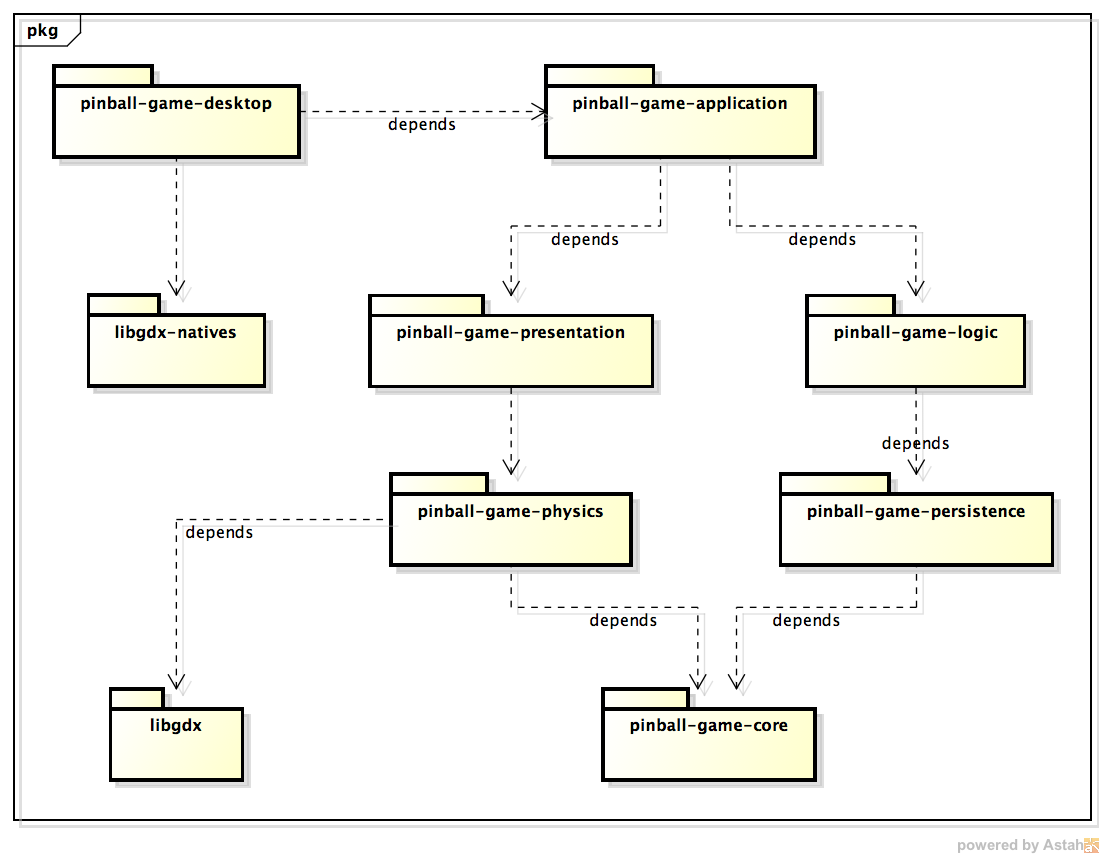
\includegraphics[width=15.5cm]{./img/package-overview.png}
	\caption[Module overview]{Module overview}
	\label{fig:module_overview}
\end{figure}

Figure~\ref{fig:module_overview} shows the modules in the pinball application. For better understanding, it contains also the modules \emph{libgdx} and \emph{libgdx-natives}.

The main modules are divided into a presentation- and a logic-branch.

\subsection{pinball-game-desktop}

This module contains the bootstrapping code (main method) for the desktop version of the application. The dependency to the \emph{libgdx-natives} includes the necessary native code in order to run on a desktop. The other parts of the application only depends on the \emph{libgdx} module, which is basically a java api for all the native code in \emph{libgdx-natives}.

\subsection{pinball-game-application}

This module contains the platform-independent implementation of the initialising and configuration of the application. It wires the presentation together with the logic in the dependency injection container.

\subsection{pinball-game-core}

This module is the base for all other modules. It defines the communication between the presentation and logic via interfaces.

\subsection{pinball-game-presentation}

This module's main responsibility is to render the screens in the OpenGL main loop.

\subsection{pinball-game-physics}

This module's main responsibility is to calculate the physics in the game.

\subsection{pinball-game-logic}

This module's main responsibility is to implement the game's logic an control the process.

\subsection{pinball-game-persistence}

This module's main responsibility is to handle access to persistent data, such as the play fields and saved simulations.

\section{Persistence}

\subsection{Play field}

\begin{figure}[h!]
	\centering
	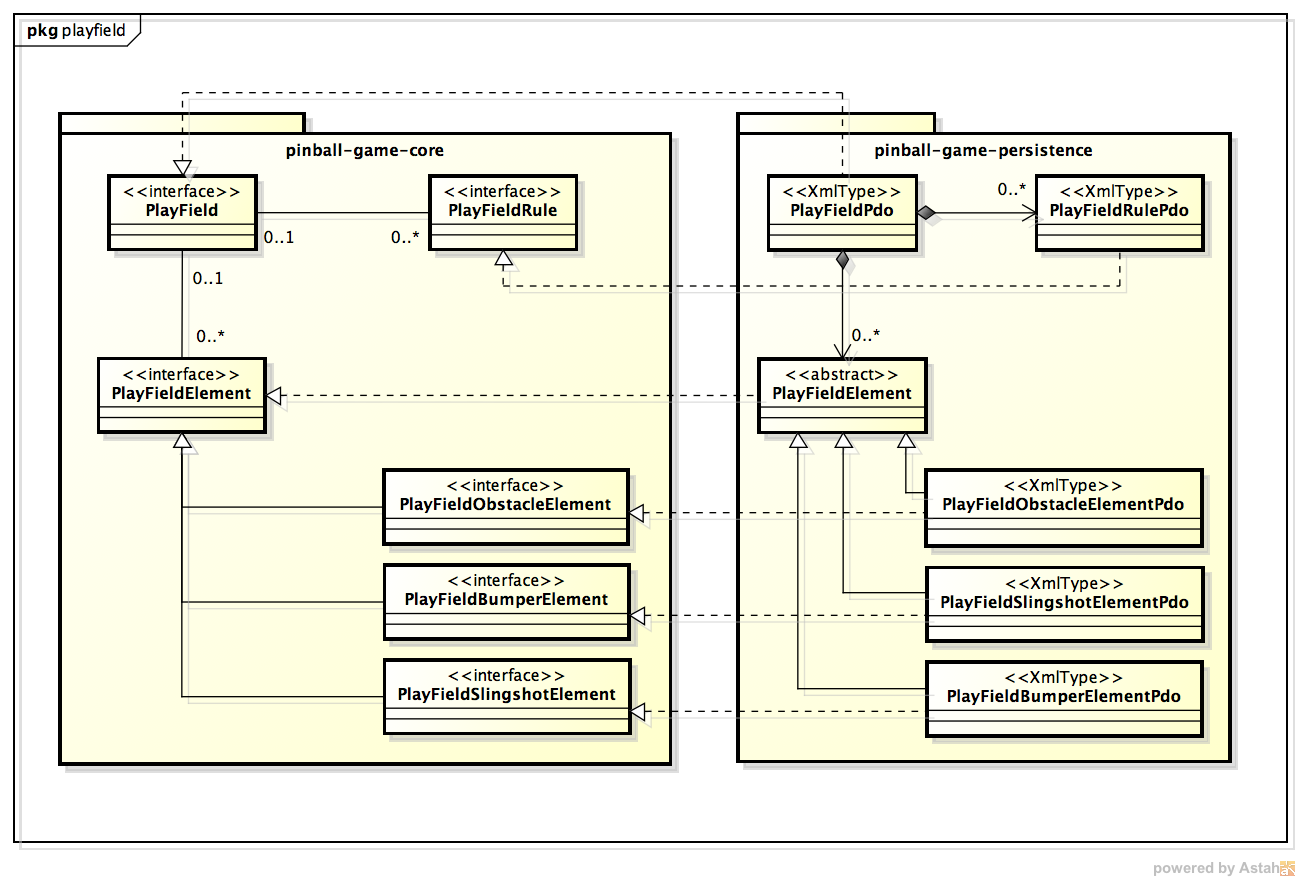
\includegraphics[width=15.5cm]{./img/persistence-playfield.png}
	\caption[Play field persistence]{Play field persistence}
	\label{fig:playfield_persistence}
\end{figure}

The play field is loaded from the XML file playfields.xml using JAXB. In the module \emph{pinball-game-core} are the interfaces used to discribe the entities which are crucial for the persistence of the data concerning a play field.

A \texttt{PlayField} can have multiple \texttt{Rule}s and it can have multiple \texttt{PlayFieldElement}s. A \texttt{PlayFieldElement} is either a \texttt{PlayFieldObstacleElement}, a \texttt{PlayFieldBumperElement} or a \texttt{PlayFieldSlingshotElement}.

In the module \emph{pinball-game-persistence} are the concrete implementations of these interfaces which are XMLTypes and have JAXB annotations which helps JAXB to insert the data of the XML file at the right place.

\subsubsection{Load playfields via JAXB}

\begin{figure}[h!]
	\centering
	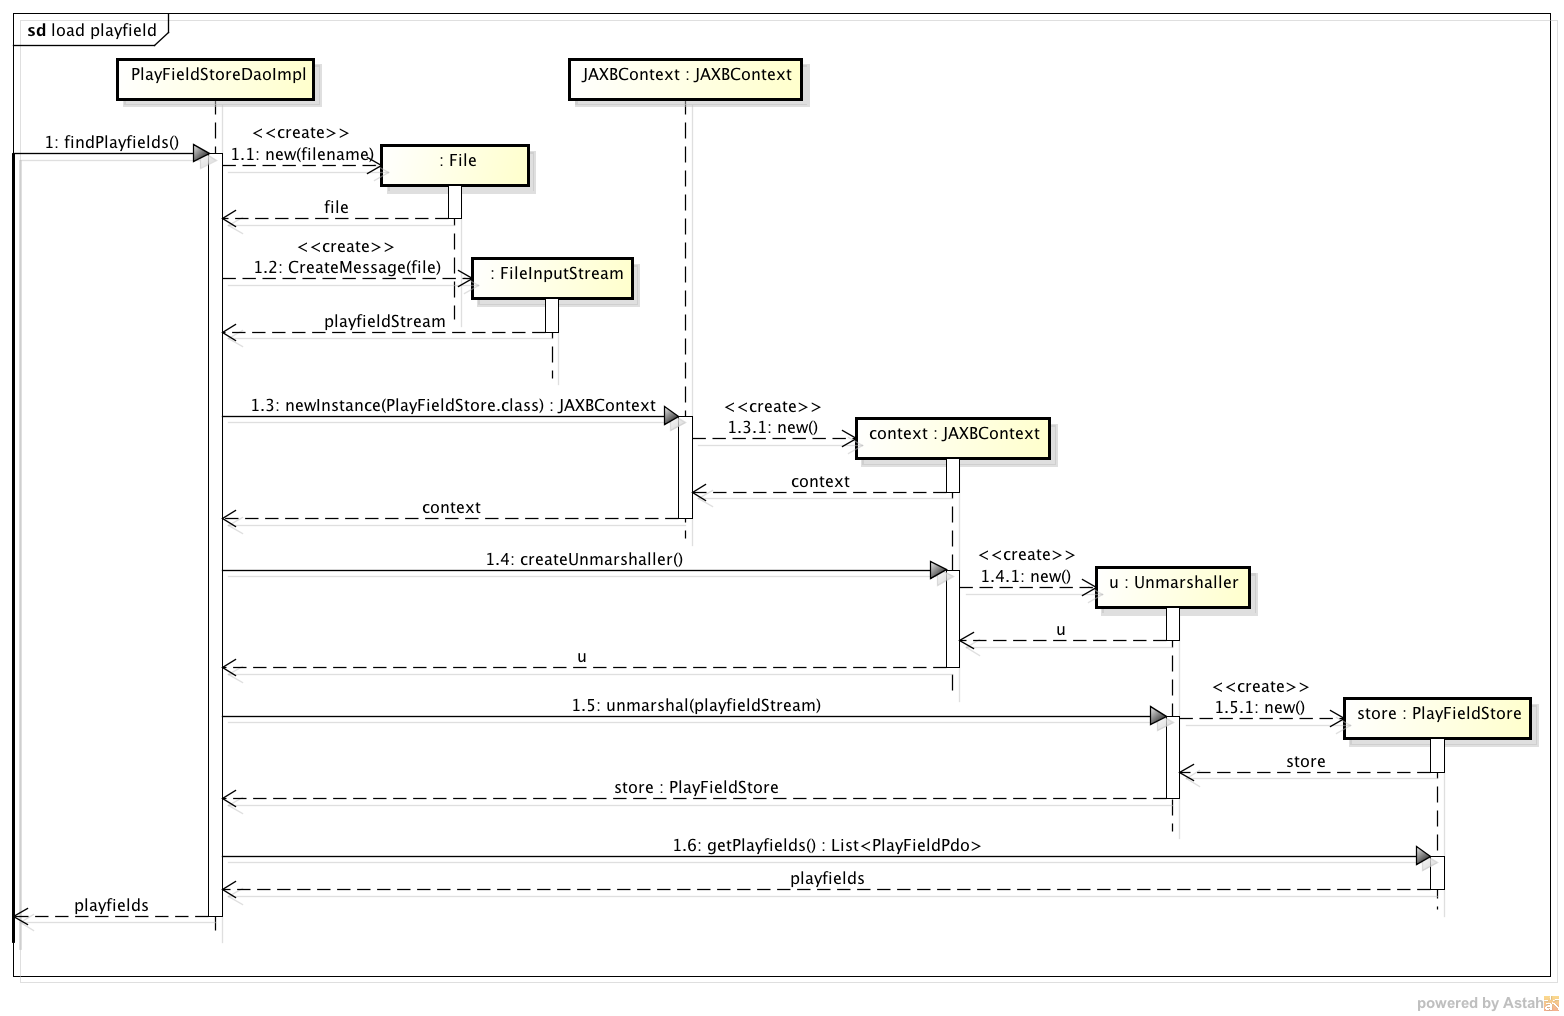
\includegraphics[width=15.5cm]{./img/jaxb-load-playfield-sd.png}
	\caption[Load play field]{Load play field with JAXB}
	\label{fig:load_playfield}
\end{figure}

This sequence diagram shows how the \emph{playfields.xml} is loaded and the \texttt{PlayFieldPdos} are generated.
We need to bind the \texttt{JAXBContext} to the class we want to unmarshal. Then we are able to create a new \texttt{Unmarshaller} which can unmarshal the \emph{playfields.xml} into an object of type \texttt{PlayFieldStore}. This object has a method getPlayfields which returns a List of \texttt{PlayFieldPdo}s.


\subsubsection{XML Schema}

The following XML schema describes the playfields.xml and is used to validate the XML file and intelligent XML editors may help the user with code completion if a XML schema is given. So the users is automatically warned if some inputs were incorrect.

\begin{lstlisting}[language=xml,label=lst:default_playfield,caption={schema for playfields.xml}]

<?xml version="1.0" encoding="UTF-8" standalone="yes"?>
<xs:schema version="1.0" targetNamespace="http://comet.m02.ch/pinball/playfield" xmlns:tns="http://comet.m02.ch/pinball/playfield" xmlns:xs="http://www.w3.org/2001/XMLSchema">

  <xs:element name="configuration" type="tns:configuration"/>

  <xs:complexType name="configuration">
    <xs:sequence>
      <xs:element name="playfields" form="qualified">
        <xs:complexType>
          <xs:sequence>
            <xs:element name="playfield" type="tns:playfield" form="qualified" maxOccurs="unbounded"/>
          </xs:sequence>
        </xs:complexType>
      </xs:element>
    </xs:sequence>
  </xs:complexType>

  <xs:complexType name="playfield">
    <xs:sequence>
      <xs:element name="name" type="xs:string" form="qualified"/>
      <xs:element name="elements" form="qualified">
        <xs:complexType>
          <xs:sequence>
            <xs:choice minOccurs="0" maxOccurs="unbounded">
              <xs:element name="bumper" type="tns:bumper" form="qualified"/>
              <xs:element name="slingshot" type="tns:slingshot" form="qualified"/>
              <xs:element name="obstacle" type="tns:obstacle" form="qualified"/>
            </xs:choice>
          </xs:sequence>
        </xs:complexType>
      </xs:element>
      <xs:element name="rules" form="qualified">
        <xs:complexType>
          <xs:sequence>
            <xs:element name="rule" type="tns:rule" form="qualified" maxOccurs="unbounded"/>
          </xs:sequence>
        </xs:complexType>
      </xs:element>
    </xs:sequence>
  </xs:complexType>

  <xs:complexType name="bumper">
    <xs:complexContent>
      <xs:extension base="tns:element">
        <xs:sequence>
          <xs:element name="radius" type="xs:float" form="qualified"/>
        </xs:sequence>
      </xs:extension>
    </xs:complexContent>
  </xs:complexType>

  <xs:complexType name="element" abstract="true">
    <xs:sequence>
      <xs:element name="id" type="xs:int" form="qualified"/>
      <xs:element name="position" type="tns:vector" form="qualified"/>
    </xs:sequence>
  </xs:complexType>

  <xs:complexType name="vector">
    <xs:sequence>
      <xs:element name="x" type="xs:float" form="qualified"/>
      <xs:element name="y" type="xs:float" form="qualified"/>
    </xs:sequence>
  </xs:complexType>

  <xs:complexType name="slingshot">
    <xs:complexContent>
      <xs:extension base="tns:element">
        <xs:sequence>
          <xs:element name="corner.a" type="tns:vector" form="qualified"/>
          <xs:element name="corner.b" type="tns:vector" form="qualified"/>
        </xs:sequence>
      </xs:extension>
    </xs:complexContent>
  </xs:complexType>

  <xs:complexType name="obstacle">
    <xs:complexContent>
      <xs:extension base="tns:element">
        <xs:sequence>
          <xs:element name="vertices" form="qualified">
            <xs:complexType>
              <xs:sequence>
                <xs:element name="vertice" type="tns:vector" form="qualified" maxOccurs="unbounded"/>
              </xs:sequence>
            </xs:complexType>
          </xs:element>
        </xs:sequence>
      </xs:extension>
    </xs:complexContent>
  </xs:complexType>

  <xs:complexType name="rule">
    <xs:sequence>
      <xs:element name="class" type="xs:string" form="qualified"/>
      <xs:element name="parameters" form="qualified">
        <xs:complexType>
          <xs:sequence>
            <xs:element name="parameter" type="xs:int" form="qualified" maxOccurs="unbounded"/>
          </xs:sequence>
        </xs:complexType>
      </xs:element>
    </xs:sequence>
  </xs:complexType>
</xs:schema>
\end{lstlisting}


\subsection{Simulation}

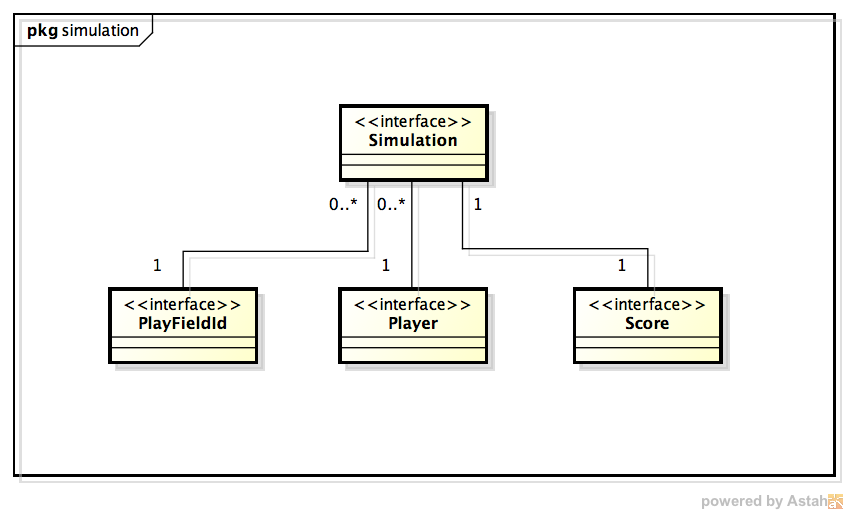
\includegraphics[width=15.5cm]{./img/persistence-simulation.png}



\section{Dependency injection}

\subsection{Why dependency injection?}

\begin{figure}[h!]
	\centering
	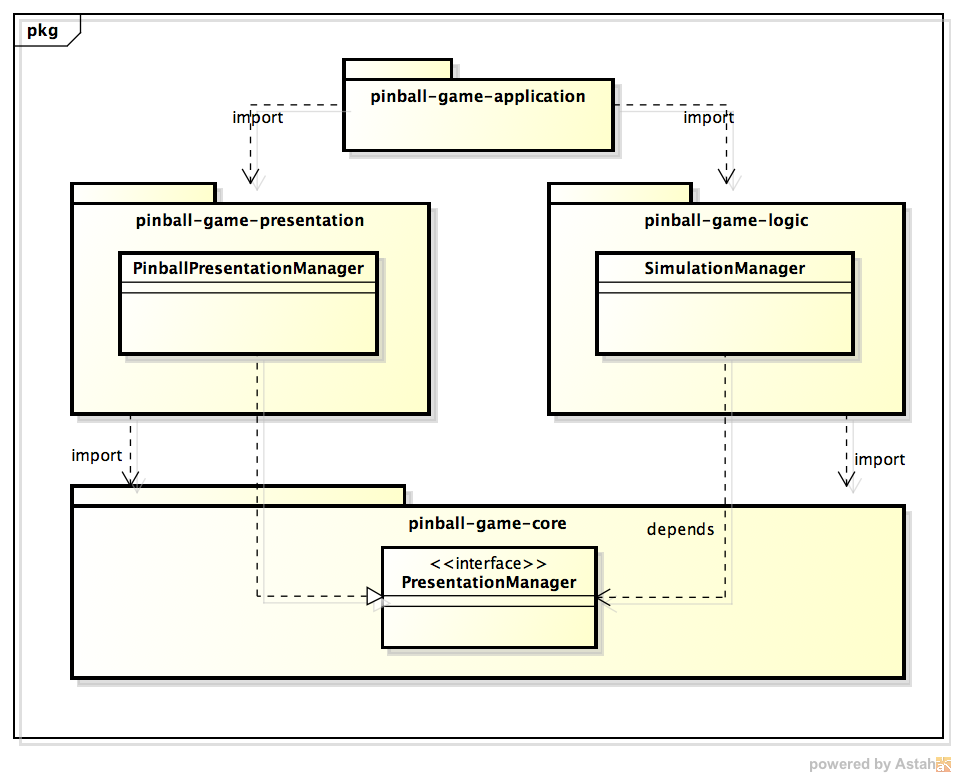
\includegraphics[width=15.5cm]{./img/dependency-injection1.png}
	\caption[System design]{System design using interfaces}
	\label{fig:dependency_injection1}
\end{figure}

\subsection{Component wiring}

\begin{figure}[h!]
	\centering
	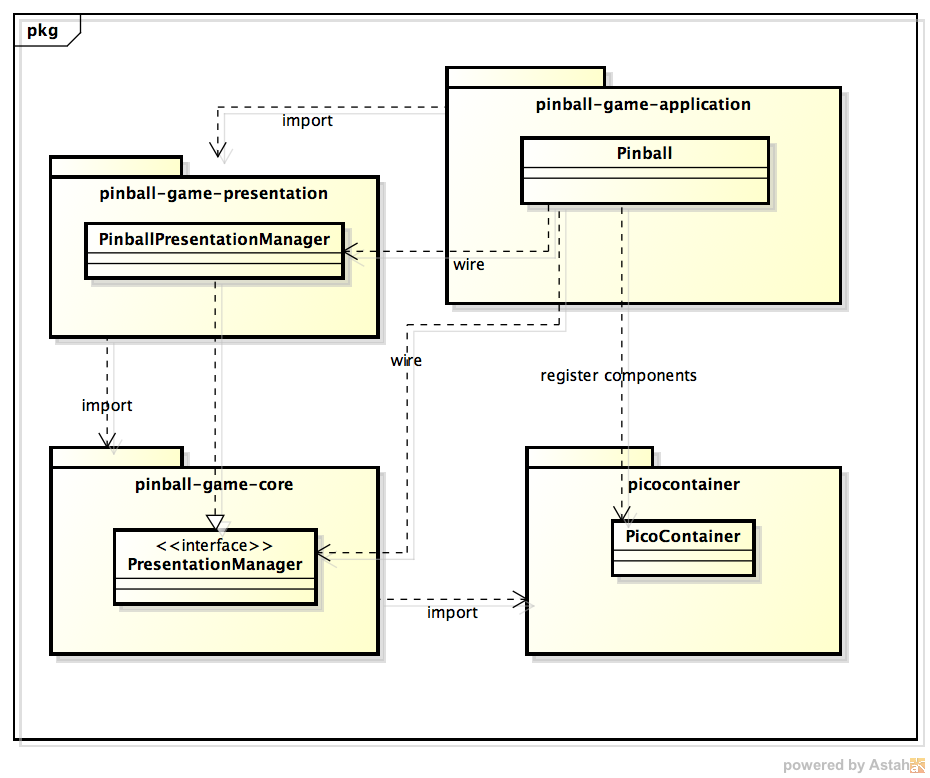
\includegraphics[width=15.5cm]{./img/dependency-injection2.png}
	\caption[Component wiring]{Component wiring}
	\label{fig:dependency_injection2}
\end{figure}


\subsection{Sequence diagram}

\begin{figure}[h!]
	\centering
	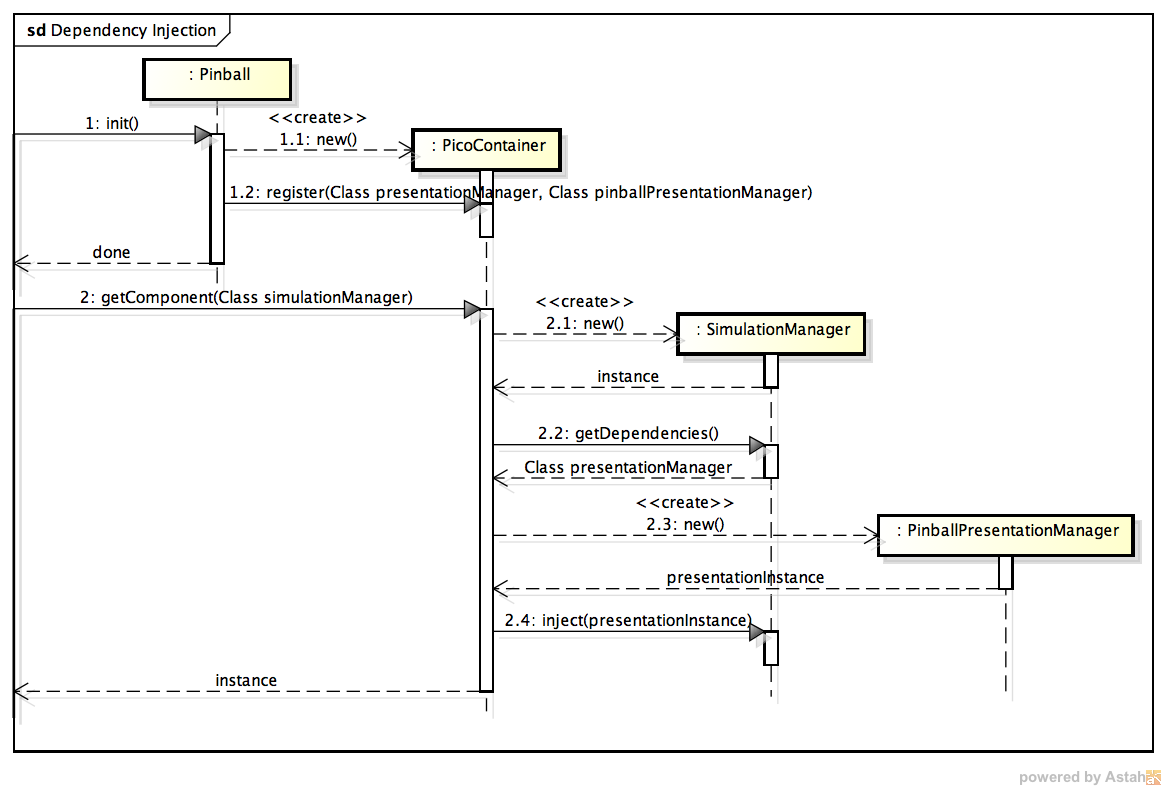
\includegraphics[width=15.5cm]{./img/dependency-injection-sd.png}
	\caption[Dependency injection]{Dependency injection}
	\label{fig:dependency_injection3}
\end{figure}

\section{Communication between modules}
\subsection{Command pattern}

\begin{figure}[h!]
	\centering
	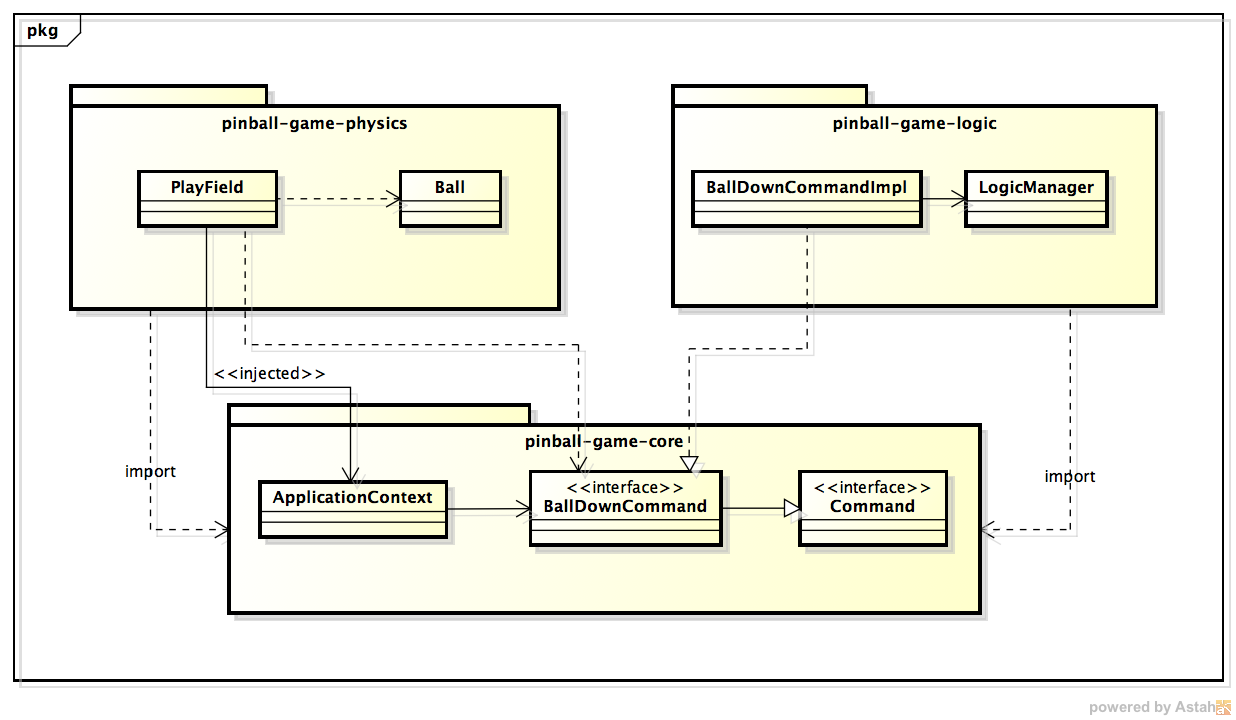
\includegraphics[width=15.5cm]{./img/command-pattern1.png}
	\caption[Command pattern]{Command pattern}
	\label{fig:command_pattern}
\end{figure}

This diagram shows how the communication between the modules is implemented with a command pattern. If the physics wants to trigger an event in the game logic, it lets the \emph{pico container} to create a new implementation of the concerning command interface. The \emph{pico container} injects the \emph{LogicManager} so the only thing left to to in the physics module is calling the method execute.


\section{State machine}

\begin{figure}[h!]
	\centering
	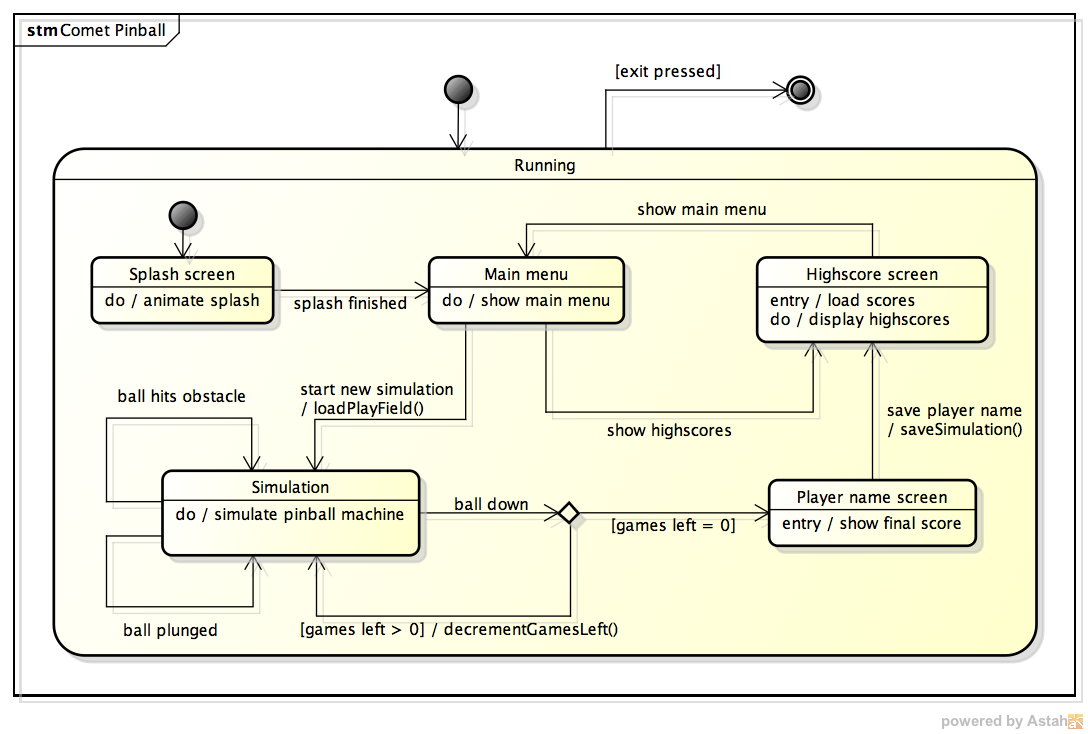
\includegraphics[width=15.5cm]{./img/state-machine.png}
	\caption[Pinball state machine]{Pinball state machine}
	\label{fig:command_pattern}
\end{figure}


\begin{figure}[h!]
	\centering
	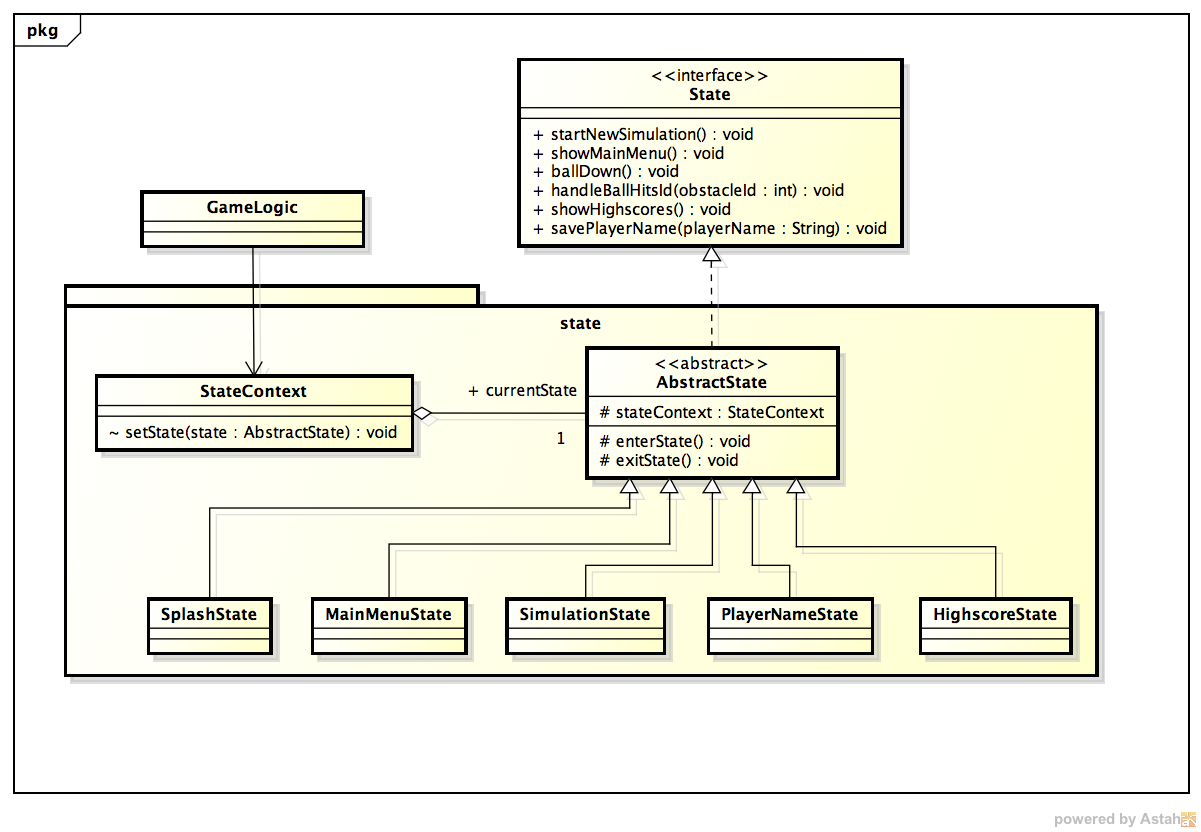
\includegraphics[width=15.5cm]{./img/state-pattern.png}
	\caption[State pattern]{State pattern}
	\label{fig:state_pattern}
\end{figure}

\end{document}
